\section{Simulations}

\subsection{Programming choices}

To implement the different schemes and run the Monte Carlo pricers, we mainly need to do a lot of additions and multiplications, and a way to generate realisations from a standard normal distribution, thus a random number generator. For those reasons, we decided to implement the code in C++, to scale the number of simulations without triggering impatience issues... and to expose the main functions in Python so they can be used in a notebook for instance, and produce visualisations quickly and easily.\\


\begin{figure}[H]
    \centering
    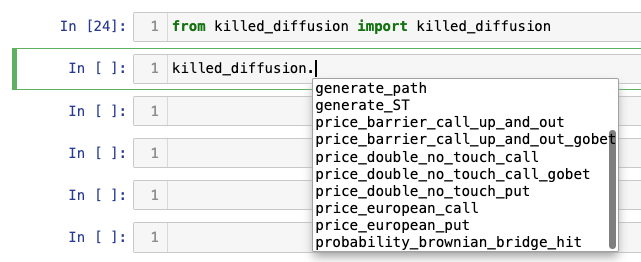
\includegraphics[width=0.6\linewidth]{img/killed_module.png}
    \caption{The killed diffusion module and available functions exposed in Python}
    \label{fig:module}
\end{figure}

The corresponding C++ files of interest lie in \texttt{src/closed_formula.cpp} and \texttt{src/montecarlo.cpp}.


For the simulations, we will consider the following set of parameters:
\begin{itemize}
    \item $S_0 = 100$
    \item $K = 100$
    \item $r = 5\%$
    \item $T = 1$
    \item $\sigma = 0.22$
    \item (number of discretization steps) $N = 500$
    \item (number of Monte Carlo simulations) $M = 15000$
    \item upper barrier $B = 120$
    \item lower barrier $L = 80$  
    
\end{itemize}

Throughout the analysis of the results, we call "MC" the discrete naive scheme while we use the name "MC - Gobet" for the continuous scheme.




\subsection{Payoffs}

\begin{figure}[H]
    \centering
    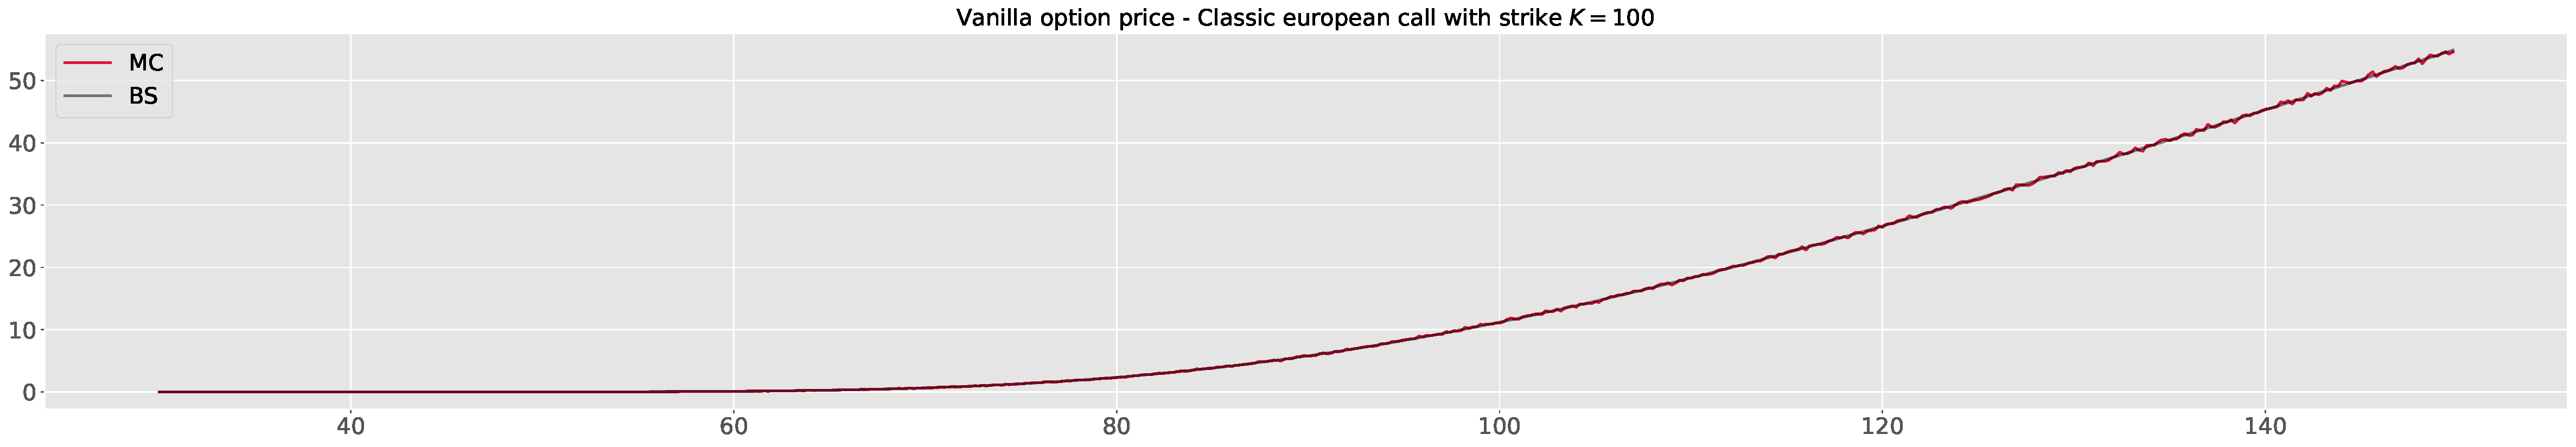
\includegraphics[width=1\linewidth]{img/vanilla_call.pdf}
    \caption{Evolution of the vanilla call option price against $S_0$}
    \label{fig:callmc}
\end{figure}

The Monte Carlo price from a discrete scheme matches very closely the theoretical price for this vanilla call.\\

Now, let's visualize the difference between classic Monte Carlo estimators using the discrete Euler scheme and the refinement introduced by Emmanuel Gobet using the law of some Brownian bridge to model the evolution between two increments.

\begin{figure}[H]
    \centering
    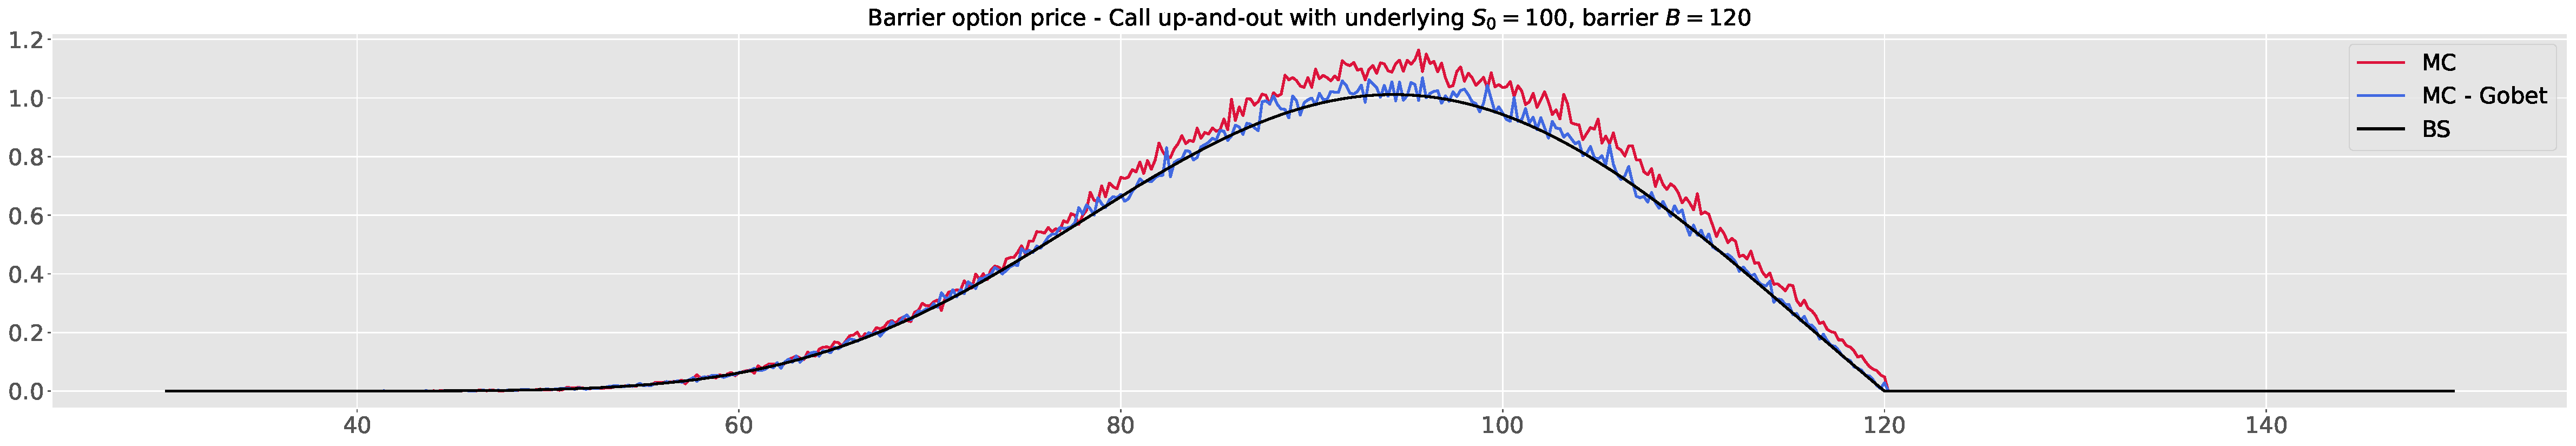
\includegraphics[width=1\linewidth]{img/cuo_mc.pdf}
    \caption{Evolution of the up-and-out barrier call option price against $S_0$}
    \label{fig:upandoutmc}
\end{figure}

The Gobet \textbf{continuous scheme appears more accurate} than a "naive" Monte Carlo pricer: indeed, the option is path-dependent and the discrete scheme leaves out some possibilities to get the diffusion killed, overestimating the survival probability of the diffusion leads to an inflated price.\\

We observe that the \textbf{price is lower than for a vanilla call option}: of course if the barrier is hit the option expires worthless. This product is interesting as it gives a different exposure than the vanilla call: there is limited upside so a trader might also express a more detailed view on volatility when buying this cheaper option.\\

Still, we observe that despite a high number of simulations and a reasonable discretization stepsize, the Monte Carlo price \textbf{lacks regularity} (the MC price gravitates around the theoretical price): if we were to be the seller of such an option, we would build a confidence interval around a given price by running the pricer several times (one instance of the Gobet method takes a little less than half a second on our personal machines) and price this uncertainty in the spread we would charge to the potential buyer -- and we certainly would not choose a geometric brownian motion dynamic for the underlying asset.

\begin{figure}[H]
    \centering
    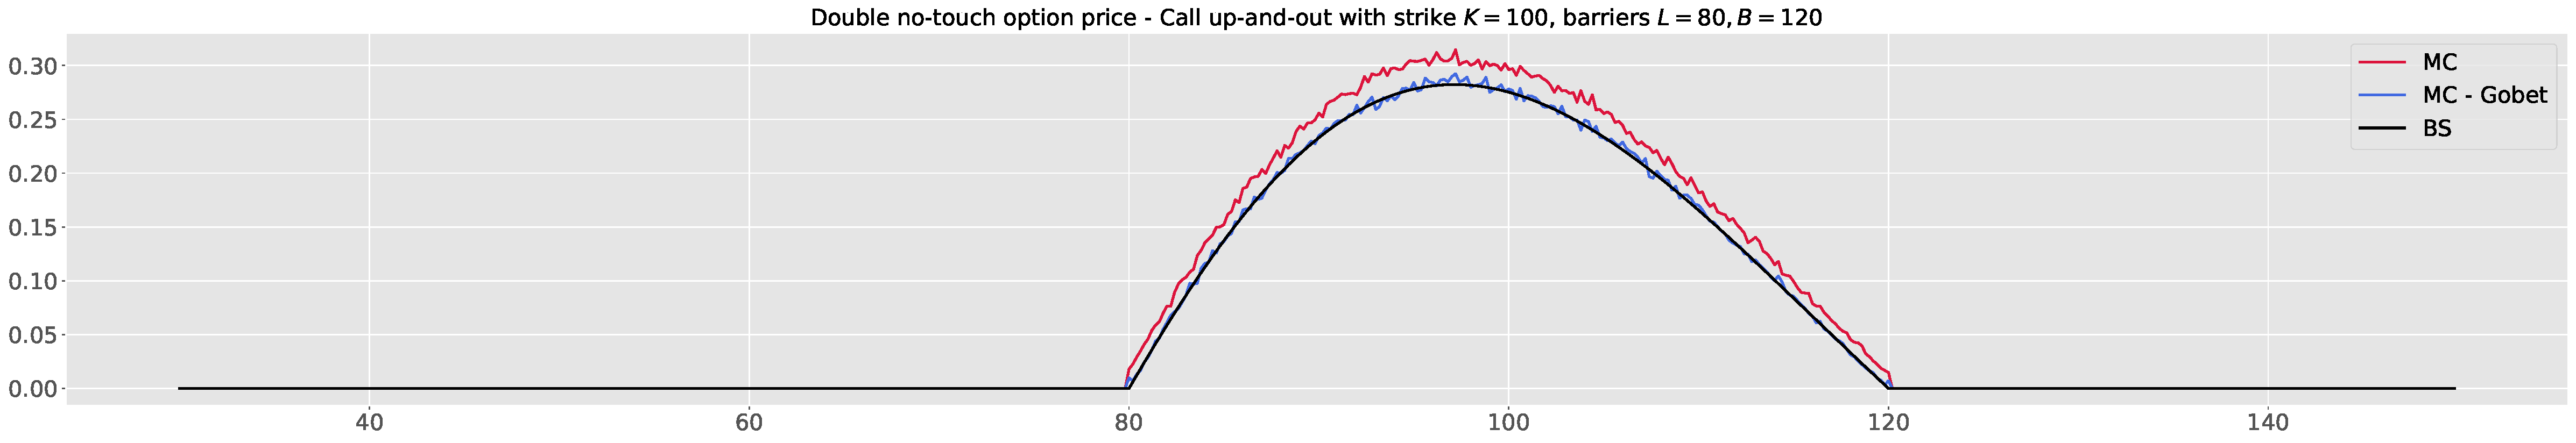
\includegraphics[width=1\linewidth]{img/dnt_mc.pdf}
    \caption{Evolution of the double no-touch option that pays $\$1$ against $S_0$}
    \label{fig:doublenotouchmc}
\end{figure}

Here we can make the same remarks as above: the continuous scheme appears to match better the theoretical price, while the discrete scheme does not account for potential death of the diffusion in-between two time-steps.\newline
Here, we see that the ATM double no-touch option would roughly pay 4-to-1, provided that the underlying asset remains between $\$80$ and $\$120$ during the whole year, knowing the asset has an annualized volatility of $22\%$.

\subsection{Killed diffusion}

% Killed diffusion (pour bien montrer la notion de temps d'arrêt et la proba de Gobet!!!)
\begin{figure}[H]
    \centering
    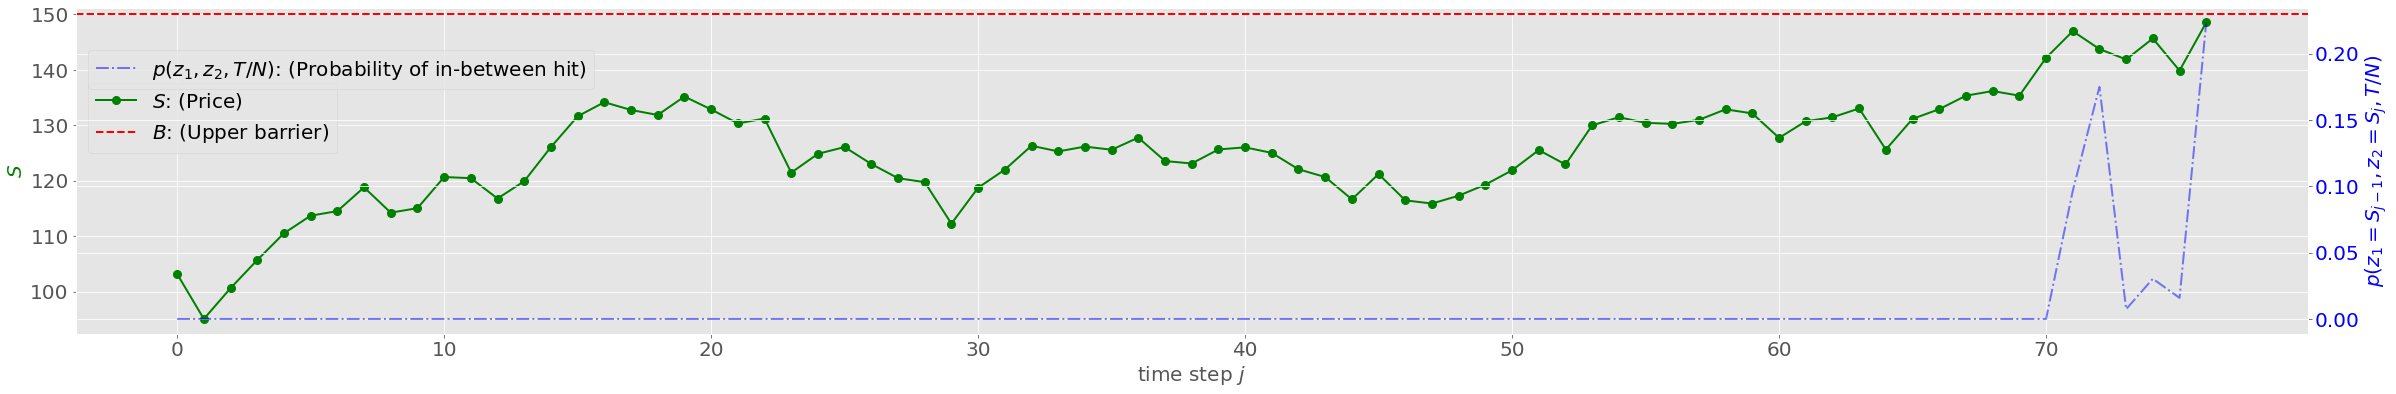
\includegraphics[width=1\linewidth]{img/barrierupandout.png}
    \caption{Killed diffusion of the underlying asset $S$ - Up-and-out barrier}
    \label{fig:barrier}
\end{figure}

\begin{figure}[H] 
    \centering
    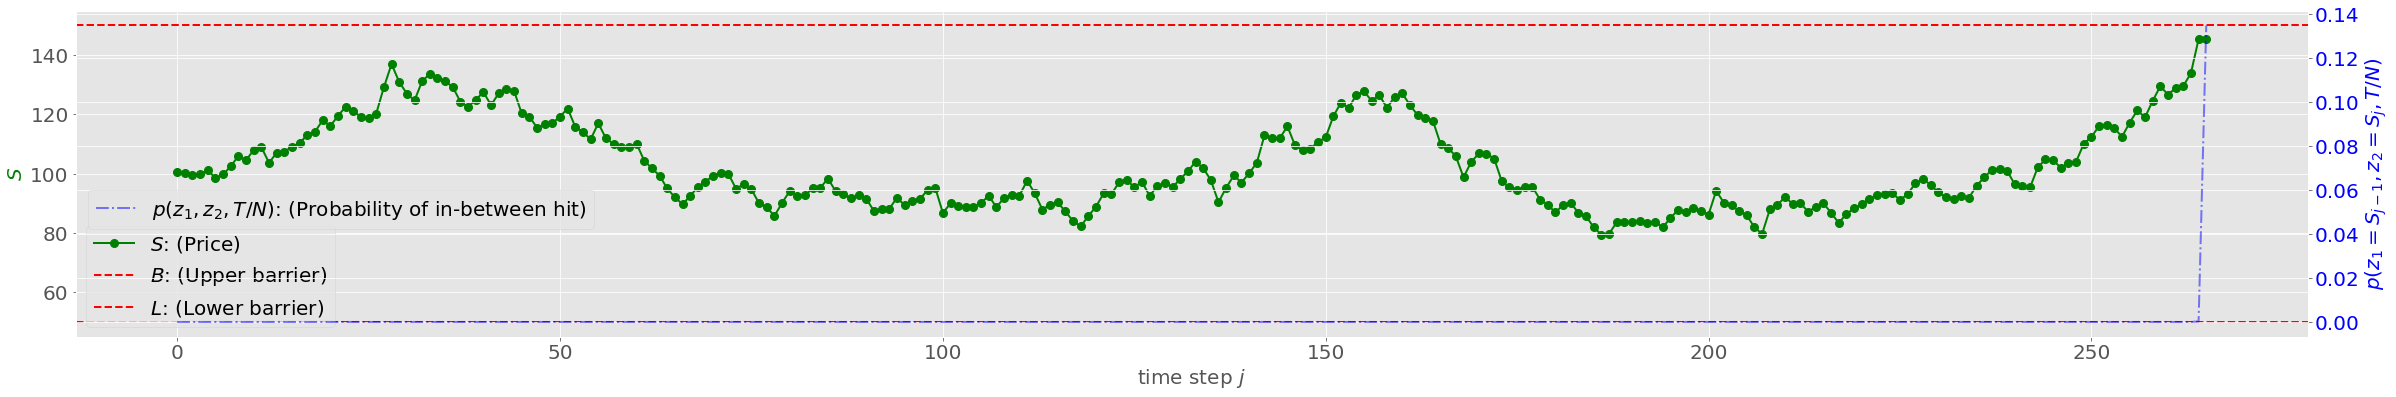
\includegraphics[width=1\linewidth]{img/doublenotouch.png}
    \caption{Killed diffusion of the underlying asset $S$ - double no-touch}
    \label{fig:doublenotouch}
\end{figure}

As we can see, the probability of hitting the barrier between two consecutive time steps rapidly grows, as the diffusion comes closer to the barrier. This contribution to the killing likelihood of the diffusion is what drives the price a bit down compared to the discrete scheme. We plot only up to the point of stopping time, \textit{i.e.} exactly where we kill the diffusion when the barrier is hit.

\subsection{Convergence}

\begin{figure}[H]
    \centering
    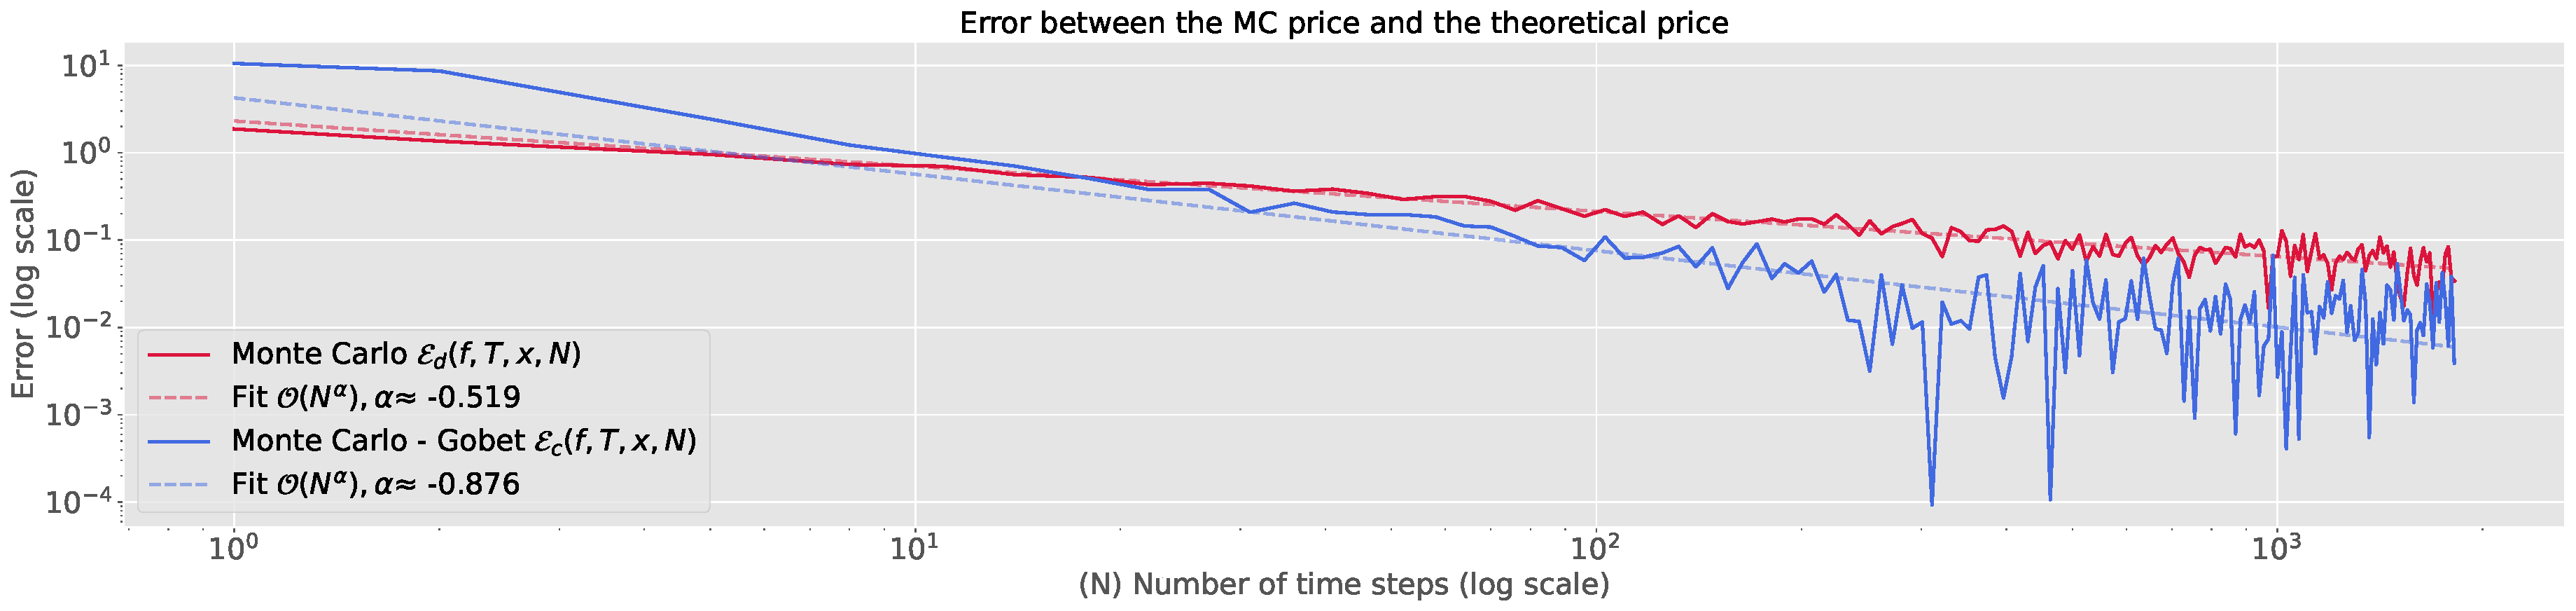
\includegraphics[width=1\linewidth]{img/convergence.pdf}
    \caption{Convergence of the errors - Discrete Euler scheme (red) vs Continuous Euler scheme (blue) with linear fits in the log-space to check for rates of convergence}
    \label{fig:convergence}
\end{figure}

To achieve this view, we sampled the two different errors by running our Monte Carlo methods using logarithmic scaling with base 1.5. This allowed to obtain estimates with varying values of $N$ ranging from 1 to roughly 2000 discretization time steps.

Note that we retrieve the convergence results of section 2. for both discrete and continuous Euler schemes. Using a linear regression on a log scale we found \textbf{empirical rates of convergence} that roughly match the one from the paper for the respective errors: 


\begin{enumerate}
    \item for the continuous Euler scheme: $\mathcal{E}_{\mathrm{c}}(f, T, x, N)=C N^{-1}+o\left(N^{-1}\right)$ provided that $f$ is a measurable function with support strictly included in $D$ (Theorem 2.1). The support condition can be weakened if $f$ is smooth enough (Theorem 2.2). Empirically we got $0.88$ for $1$ theoretically.

    \item for the discrete Euler scheme: $\mathcal{E}_{\mathrm{d}}(f, T, x, N)=O\left(N^{-1 / 2}\right)$ for functions $f$ satisfying analogous hypotheses as before (Theorem 2.3). The rate $N^{-1 / 2}$ is optimal and intrinsic to the choice of a discrete killing time (Theorem 2.4). Empirically we got $0.52$ for $0.5$ theoretically.

\end{enumerate}

In the case of our up-and-out barrier call option, $f$ is defined as $x \mapsto (x-K)_{+}$, for the double no-touch option it simply is $x \mapsto 1$, or any amount that the counterparty agrees to pay upon meeting the staying in-between the barriers during the lifetime of the option condition.